\documentclass{standalone}
\usepackage{tikz}
\usetikzlibrary{patterns, positioning}


\begin{document}
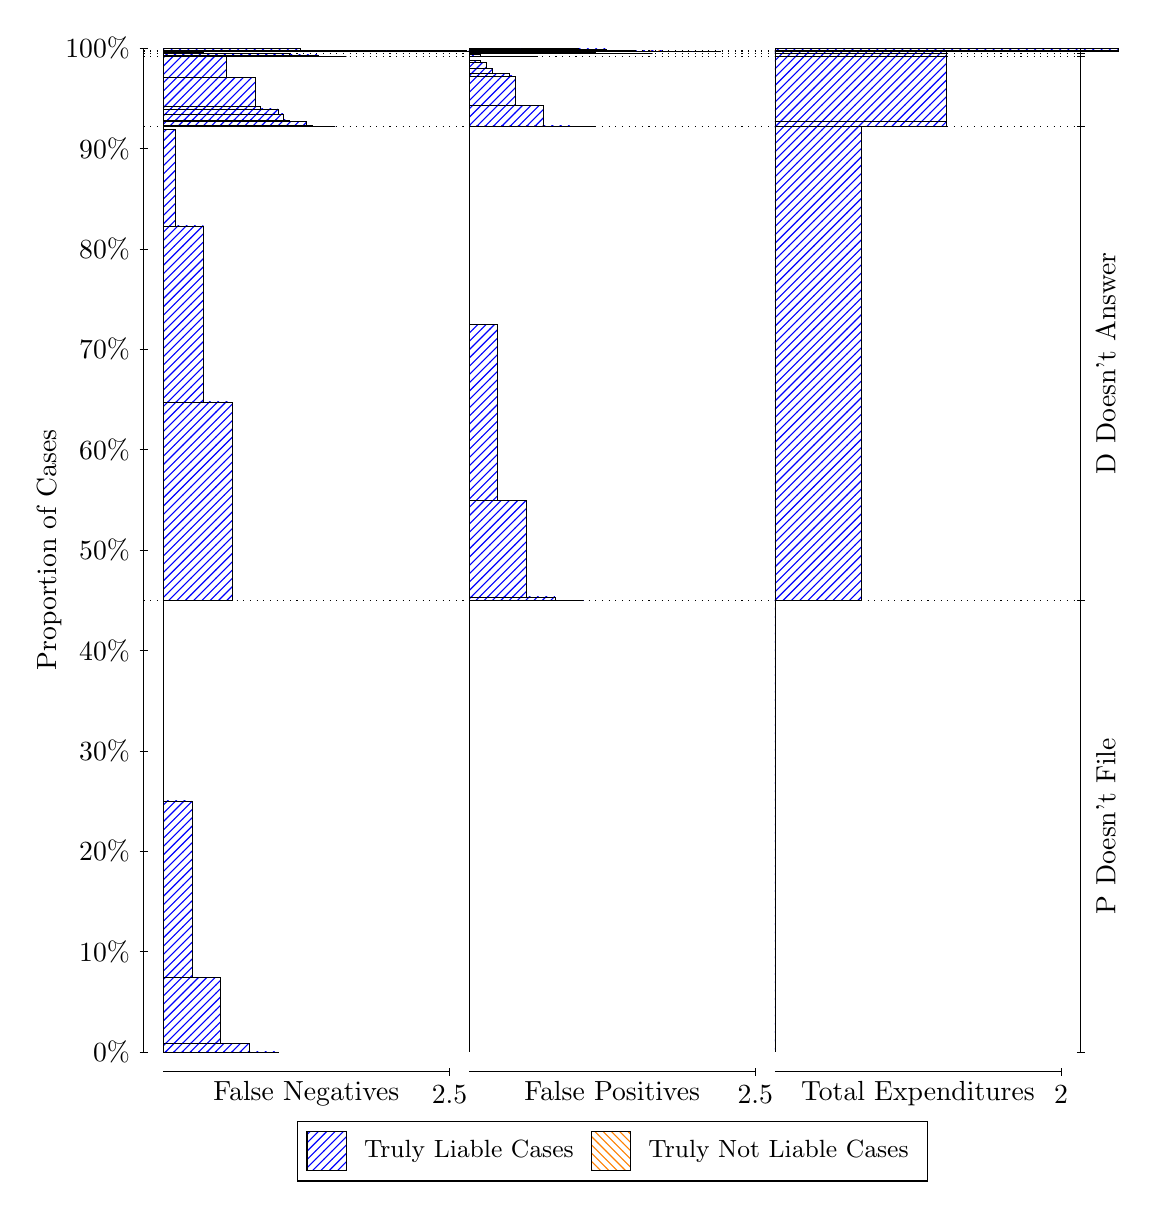
\begin{tikzpicture}
\draw[black, very thin] (1.5,1.75) -- (1.5,14.5);
\node[rotate=90, text=black, anchor=center] at (0.3, 8.125) {Proportion of Cases};
\draw[black, very thin] (1.45,1.75) -- (1.55,1.75);
\node[text=black, anchor=east] at (1.45, 1.75) {0\%};
\draw[black, very thin] (1.45,3.025) -- (1.55,3.025);
\node[text=black, anchor=east] at (1.45, 3.025) {10\%};
\draw[black, very thin] (1.45,4.3) -- (1.55,4.3);
\node[text=black, anchor=east] at (1.45, 4.3) {20\%};
\draw[black, very thin] (1.45,5.575) -- (1.55,5.575);
\node[text=black, anchor=east] at (1.45, 5.575) {30\%};
\draw[black, very thin] (1.45,6.85) -- (1.55,6.85);
\node[text=black, anchor=east] at (1.45, 6.85) {40\%};
\draw[black, very thin] (1.45,8.125) -- (1.55,8.125);
\node[text=black, anchor=east] at (1.45, 8.125) {50\%};
\draw[black, very thin] (1.45,9.4) -- (1.55,9.4);
\node[text=black, anchor=east] at (1.45, 9.4) {60\%};
\draw[black, very thin] (1.45,10.675) -- (1.55,10.675);
\node[text=black, anchor=east] at (1.45, 10.675) {70\%};
\draw[black, very thin] (1.45,11.95) -- (1.55,11.95);
\node[text=black, anchor=east] at (1.45, 11.95) {80\%};
\draw[black, very thin] (1.45,13.225) -- (1.55,13.225);
\node[text=black, anchor=east] at (1.45, 13.225) {90\%};
\draw[black, very thin] (1.45,14.5) -- (1.55,14.5);
\node[text=black, anchor=east] at (1.45, 14.5) {100\%};

\draw[black, very thin] (13.4,1.75) -- (13.4,14.5);
\draw[black, very thin] (13.35,1.75) -- (13.45,1.75);
\node[anchor=west] at (13.35, 1.75) {};
\draw[black, very thin] (13.35,7.487) -- (13.45,7.487);
\node[anchor=west] at (13.35, 7.487) {};
\draw[black, very thin] (13.35,13.509) -- (13.45,13.509);
\node[anchor=west] at (13.35, 13.509) {};
\draw[black, very thin] (13.35,14.396) -- (13.45,14.396);
\node[anchor=west] at (13.35, 14.396) {};
\draw[black, very thin] (13.35,14.435) -- (13.45,14.435);
\node[anchor=west] at (13.35, 14.435) {};
\draw[black, very thin] (13.35,14.462) -- (13.45,14.462);
\node[anchor=west] at (13.35, 14.462) {};
\draw[black, very thin] (13.35,14.5) -- (13.45,14.5);
\node[anchor=west] at (13.35, 14.5) {};

\draw[black, very thin, pattern color=blue, pattern=north east lines] (1.75,1.75) rectangle (3.2033,1.751);
\draw[black, very thin, pattern color=blue, pattern=north east lines] (1.75,1.751) rectangle (2.84,1.8549);
\draw[black, very thin, pattern color=blue, pattern=north east lines] (1.75,1.8549) rectangle (2.4767,2.6947);
\draw[black, very thin, pattern color=blue, pattern=north east lines] (1.75,2.6947) rectangle (2.1133,4.94);
\draw[black, very thin, pattern color=orange, pattern=north west lines] (1.75,4.94) rectangle (1.75,4.94);
\draw[black, very thin, pattern color=blue, pattern=north east lines] (1.75,4.94) rectangle (1.75,7.487);
\draw[black, very thin, pattern color=blue, pattern=north east lines] (1.75,7.487) rectangle (2.622,10.007);
\draw[black, very thin, pattern color=blue, pattern=north east lines] (1.75,10.007) rectangle (2.2587,12.242);
\draw[black, very thin, pattern color=blue, pattern=north east lines] (1.75,12.242) rectangle (1.8953,13.467);
\draw[black, very thin, pattern color=orange, pattern=north west lines] (1.75,13.467) rectangle (1.75,13.467);
\draw[black, very thin, pattern color=blue, pattern=north east lines] (1.75,13.467) rectangle (1.75,13.509);
\draw[black, very thin, pattern color=blue, pattern=north east lines] (1.75,13.509) rectangle (3.93,13.509);
\draw[black, very thin, pattern color=blue, pattern=north east lines] (1.75,13.509) rectangle (3.6393,13.513);
\draw[black, very thin, pattern color=blue, pattern=north east lines] (1.75,13.513) rectangle (3.5667,13.565);
\draw[black, very thin, pattern color=blue, pattern=north east lines] (1.75,13.565) rectangle (3.3487,13.588);
\draw[black, very thin, pattern color=blue, pattern=north east lines] (1.75,13.588) rectangle (3.276,13.664);
\draw[black, very thin, pattern color=blue, pattern=north east lines] (1.75,13.664) rectangle (3.2033,13.727);
\draw[black, very thin, pattern color=blue, pattern=north east lines] (1.75,13.727) rectangle (2.9853,13.76);
\draw[black, very thin, pattern color=blue, pattern=north east lines] (1.75,13.76) rectangle (2.9127,14.131);
\draw[black, very thin, pattern color=blue, pattern=north east lines] (1.75,14.131) rectangle (2.84,14.131);
\draw[black, very thin, pattern color=blue, pattern=north east lines] (1.75,14.131) rectangle (2.622,14.132);
\draw[black, very thin, pattern color=blue, pattern=north east lines] (1.75,14.132) rectangle (2.5493,14.393);
\draw[black, very thin, pattern color=blue, pattern=north east lines] (1.75,14.393) rectangle (2.4767,14.393);
\draw[black, very thin, pattern color=blue, pattern=north east lines] (1.75,14.393) rectangle (2.2587,14.393);
\draw[black, very thin, pattern color=blue, pattern=north east lines] (1.75,14.393) rectangle (2.186,14.396);
\draw[black, very thin, pattern color=blue, pattern=north east lines] (1.75,14.396) rectangle (1.8953,14.396);
\draw[black, very thin, pattern color=orange, pattern=north west lines] (1.75,14.396) rectangle (1.75,14.396);
\draw[black, very thin, pattern color=blue, pattern=north east lines] (1.75,14.396) rectangle (4.0753,14.396);
\draw[black, very thin, pattern color=blue, pattern=north east lines] (1.75,14.396) rectangle (3.712,14.414);
\draw[black, very thin, pattern color=blue, pattern=north east lines] (1.75,14.414) rectangle (3.3487,14.435);
\draw[black, very thin, pattern color=blue, pattern=north east lines] (1.75,14.435) rectangle (2.9853,14.435);
\draw[black, very thin, pattern color=blue, pattern=north east lines] (1.75,14.435) rectangle (2.622,14.435);
\draw[black, very thin, pattern color=orange, pattern=north west lines] (1.75,14.435) rectangle (1.75,14.435);
\draw[black, very thin, pattern color=blue, pattern=north east lines] (1.75,14.435) rectangle (2.622,14.436);
\draw[black, very thin, pattern color=blue, pattern=north east lines] (1.75,14.436) rectangle (2.2587,14.452);
\draw[black, very thin, pattern color=blue, pattern=north east lines] (1.75,14.452) rectangle (1.8953,14.462);
\draw[black, very thin, pattern color=orange, pattern=north west lines] (1.75,14.462) rectangle (1.75,14.462);
\draw[black, very thin, pattern color=blue, pattern=north east lines] (1.75,14.462) rectangle (1.75,14.462);
\draw[black, very thin, pattern color=blue, pattern=north east lines] (1.75,14.462) rectangle (6.6913,14.462);
\draw[black, very thin, pattern color=blue, pattern=north east lines] (1.75,14.462) rectangle (6.328,14.462);
\draw[black, very thin, pattern color=blue, pattern=north east lines] (1.75,14.462) rectangle (5.9647,14.463);
\draw[black, very thin, pattern color=blue, pattern=north east lines] (1.75,14.463) rectangle (5.6013,14.467);
\draw[black, very thin, pattern color=blue, pattern=north east lines] (1.75,14.467) rectangle (5.238,14.467);
\draw[black, very thin, pattern color=blue, pattern=north east lines] (1.75,14.467) rectangle (4.8747,14.467);
\draw[black, very thin, pattern color=blue, pattern=north east lines] (1.75,14.467) rectangle (4.584,14.467);
\draw[black, very thin, pattern color=blue, pattern=north east lines] (1.75,14.467) rectangle (4.2207,14.468);
\draw[black, very thin, pattern color=blue, pattern=north east lines] (1.75,14.468) rectangle (3.8573,14.472);
\draw[black, very thin, pattern color=blue, pattern=north east lines] (1.75,14.472) rectangle (3.494,14.491);
\draw[black, very thin, pattern color=blue, pattern=north east lines] (1.75,14.491) rectangle (3.1307,14.5);
\draw[black, very thin, pattern color=blue, pattern=north east lines] (1.75,14.5) rectangle (2.7673,14.5);
\draw[black, very thin, pattern color=blue, pattern=north east lines] (1.75,14.5) rectangle (2.404,14.5);
\draw[black, very thin, pattern color=blue, pattern=north east lines] (1.75,14.5) rectangle (2.0407,14.5);
\draw[black, very thin, pattern color=orange, pattern=north west lines] (1.75,14.5) rectangle (1.75,14.5);
\draw[black, very thin, pattern color=orange, pattern=north west lines] (5.6333,1.75) rectangle (5.6333,1.75);
\draw[black, very thin, pattern color=blue, pattern=north east lines] (5.6333,1.75) rectangle (5.6333,7.487);
\draw[black, very thin, pattern color=orange, pattern=north west lines] (5.6333,7.487) rectangle (7.0867,7.487);
\draw[black, very thin, pattern color=blue, pattern=north east lines] (5.6333,7.487) rectangle (7.0867,7.487);
\draw[black, very thin, pattern color=blue, pattern=north east lines] (5.6333,7.487) rectangle (6.7233,7.5291);
\draw[black, very thin, pattern color=blue, pattern=north east lines] (5.6333,7.5291) rectangle (6.36,8.7537);
\draw[black, very thin, pattern color=blue, pattern=north east lines] (5.6333,8.7537) rectangle (5.9967,10.989);
\draw[black, very thin, pattern color=blue, pattern=north east lines] (5.6333,10.989) rectangle (5.6333,13.509);
\draw[black, very thin, pattern color=orange, pattern=north west lines] (5.6333,13.509) rectangle (7.232,13.509);
\draw[black, very thin, pattern color=blue, pattern=north east lines] (5.6333,13.509) rectangle (7.232,13.509);
\draw[black, very thin, pattern color=orange, pattern=north west lines] (5.6333,13.509) rectangle (6.9413,13.509);
\draw[black, very thin, pattern color=blue, pattern=north east lines] (5.6333,13.509) rectangle (6.9413,13.512);
\draw[black, very thin, pattern color=blue, pattern=north east lines] (5.6333,13.512) rectangle (6.8687,13.512);
\draw[black, very thin, pattern color=orange, pattern=north west lines] (5.6333,13.512) rectangle (6.6507,13.512);
\draw[black, very thin, pattern color=blue, pattern=north east lines] (5.6333,13.512) rectangle (6.6507,13.512);
\draw[black, very thin, pattern color=blue, pattern=north east lines] (5.6333,13.512) rectangle (6.578,13.773);
\draw[black, very thin, pattern color=blue, pattern=north east lines] (5.6333,13.773) rectangle (6.5053,13.774);
\draw[black, very thin, pattern color=blue, pattern=north east lines] (5.6333,13.774) rectangle (6.2873,13.775);
\draw[black, very thin, pattern color=blue, pattern=north east lines] (5.6333,13.775) rectangle (6.2147,14.145);
\draw[black, very thin, pattern color=blue, pattern=north east lines] (5.6333,14.145) rectangle (6.142,14.179);
\draw[black, very thin, pattern color=blue, pattern=north east lines] (5.6333,14.179) rectangle (5.924,14.242);
\draw[black, very thin, pattern color=blue, pattern=north east lines] (5.6333,14.242) rectangle (5.8513,14.317);
\draw[black, very thin, pattern color=blue, pattern=north east lines] (5.6333,14.317) rectangle (5.7787,14.341);
\draw[black, very thin, pattern color=blue, pattern=north east lines] (5.6333,14.341) rectangle (5.6333,14.396);
\draw[black, very thin, pattern color=orange, pattern=north west lines] (5.6333,14.396) rectangle (6.5053,14.396);
\draw[black, very thin, pattern color=blue, pattern=north east lines] (5.6333,14.396) rectangle (6.5053,14.396);
\draw[black, very thin, pattern color=blue, pattern=north east lines] (5.6333,14.396) rectangle (6.142,14.396);
\draw[black, very thin, pattern color=blue, pattern=north east lines] (5.6333,14.396) rectangle (5.7787,14.418);
\draw[black, very thin, pattern color=blue, pattern=north east lines] (5.6333,14.418) rectangle (5.6333,14.435);
\draw[black, very thin, pattern color=orange, pattern=north west lines] (5.6333,14.435) rectangle (7.9587,14.435);
\draw[black, very thin, pattern color=blue, pattern=north east lines] (5.6333,14.435) rectangle (7.9587,14.435);
\draw[black, very thin, pattern color=blue, pattern=north east lines] (5.6333,14.435) rectangle (7.5953,14.436);
\draw[black, very thin, pattern color=blue, pattern=north east lines] (5.6333,14.436) rectangle (7.232,14.446);
\draw[black, very thin, pattern color=blue, pattern=north east lines] (5.6333,14.446) rectangle (6.8687,14.462);
\draw[black, very thin, pattern color=blue, pattern=north east lines] (5.6333,14.462) rectangle (6.5053,14.462);
\draw[black, very thin, pattern color=orange, pattern=north west lines] (5.6333,14.462) rectangle (8.8307,14.462);
\draw[black, very thin, pattern color=blue, pattern=north east lines] (5.6333,14.462) rectangle (8.8307,14.462);
\draw[black, very thin, pattern color=blue, pattern=north east lines] (5.6333,14.462) rectangle (8.4673,14.462);
\draw[black, very thin, pattern color=orange, pattern=north west lines] (5.6333,14.462) rectangle (8.4673,14.462);
\draw[black, very thin, pattern color=blue, pattern=north east lines] (5.6333,14.462) rectangle (8.4673,14.462);
\draw[black, very thin, pattern color=blue, pattern=north east lines] (5.6333,14.462) rectangle (8.104,14.463);
\draw[black, very thin, pattern color=orange, pattern=north west lines] (5.6333,14.463) rectangle (8.104,14.463);
\draw[black, very thin, pattern color=blue, pattern=north east lines] (5.6333,14.463) rectangle (8.104,14.463);
\draw[black, very thin, pattern color=blue, pattern=north east lines] (5.6333,14.463) rectangle (7.7407,14.467);
\draw[black, very thin, pattern color=orange, pattern=north west lines] (5.6333,14.467) rectangle (7.7407,14.467);
\draw[black, very thin, pattern color=blue, pattern=north east lines] (5.6333,14.467) rectangle (7.7407,14.471);
\draw[black, very thin, pattern color=blue, pattern=north east lines] (5.6333,14.471) rectangle (7.3773,14.472);
\draw[black, very thin, pattern color=blue, pattern=north east lines] (5.6333,14.472) rectangle (7.3773,14.49);
\draw[black, very thin, pattern color=blue, pattern=north east lines] (5.6333,14.49) rectangle (7.014,14.494);
\draw[black, very thin, pattern color=blue, pattern=north east lines] (5.6333,14.494) rectangle (6.6507,14.495);
\draw[black, very thin, pattern color=blue, pattern=north east lines] (5.6333,14.495) rectangle (6.2873,14.495);
\draw[black, very thin, pattern color=orange, pattern=north west lines] (5.6333,14.495) rectangle (5.9967,14.495);
\draw[black, very thin, pattern color=blue, pattern=north east lines] (5.6333,14.495) rectangle (5.9967,14.495);
\draw[black, very thin, pattern color=orange, pattern=north west lines] (5.6333,14.495) rectangle (5.6333,14.495);
\draw[black, very thin, pattern color=blue, pattern=north east lines] (5.6333,14.495) rectangle (5.6333,14.5);
\draw[black, very thin, pattern color=orange, pattern=north west lines] (9.5167,1.75) rectangle (9.5167,1.75);
\draw[black, very thin, pattern color=blue, pattern=north east lines] (9.5167,1.75) rectangle (9.5167,7.487);
\draw[black, very thin, pattern color=orange, pattern=north west lines] (9.5167,7.487) rectangle (10.607,7.487);
\draw[black, very thin, pattern color=blue, pattern=north east lines] (9.5167,7.487) rectangle (10.607,13.509);
\draw[black, very thin, pattern color=orange, pattern=north west lines] (9.5167,13.509) rectangle (11.697,13.509);
\draw[black, very thin, pattern color=blue, pattern=north east lines] (9.5167,13.509) rectangle (11.697,13.567);
\draw[black, very thin, pattern color=orange, pattern=north west lines] (9.5167,13.567) rectangle (11.697,13.567);
\draw[black, very thin, pattern color=blue, pattern=north east lines] (9.5167,13.567) rectangle (11.697,14.396);
\draw[black, very thin, pattern color=orange, pattern=north west lines] (9.5167,14.396) rectangle (11.697,14.396);
\draw[black, very thin, pattern color=blue, pattern=north east lines] (9.5167,14.396) rectangle (11.697,14.435);
\draw[black, very thin, pattern color=orange, pattern=north west lines] (9.5167,14.435) rectangle (11.697,14.435);
\draw[black, very thin, pattern color=blue, pattern=north east lines] (9.5167,14.435) rectangle (11.697,14.462);
\draw[black, very thin, pattern color=orange, pattern=north west lines] (9.5167,14.462) rectangle (13.877,14.462);
\draw[black, very thin, pattern color=blue, pattern=north east lines] (9.5167,14.462) rectangle (13.877,14.467);
\draw[black, very thin, pattern color=orange, pattern=north west lines] (9.5167,14.467) rectangle (13.877,14.467);
\draw[black, very thin, pattern color=blue, pattern=north east lines] (9.5167,14.467) rectangle (13.877,14.5);
\draw[black, dotted] (1.5,7.487) -- (13.4,7.487);
\draw[black, dotted] (1.5,13.509) -- (13.4,13.509);
\draw[black, dotted] (1.5,14.396) -- (13.4,14.396);
\draw[black, dotted] (1.5,14.435) -- (13.4,14.435);
\draw[black, dotted] (1.5,14.462) -- (13.4,14.462);
\draw[black, very thin] (1.75,1.5) -- (5.3833,1.5);
\node[text=black, anchor=north] at (3.5667, 1.5) {False Negatives};
\draw[black, very thin] (5.3833,1.45) -- (5.3833,1.55);
\node[text=black, anchor=north] at (5.3833, 1.45) {2.5};

\draw[black, very thin] (5.6333,1.5) -- (9.2667,1.5);
\node[text=black, anchor=north] at (7.45, 1.5) {False Positives};
\draw[black, very thin] (9.2667,1.45) -- (9.2667,1.55);
\node[text=black, anchor=north] at (9.2667, 1.45) {2.5};

\draw[black, very thin] (9.5167,1.5) -- (13.15,1.5);
\node[text=black, anchor=north] at (11.333, 1.5) {Total Expenditures};
\draw[black, very thin] (13.15,1.45) -- (13.15,1.55);
\node[text=black, anchor=north] at (13.15, 1.45) {2};

\node[text=black, centered, rotate=90] at (13.72, 4.6185) {P Doesn't File};
\node[text=black, centered, rotate=90] at (13.72, 10.498) {D Doesn't Answer};





\draw (7.449999999999999,1.5) node[draw=none] (baseCoordinate) {};
\begin{scope}[align=center]
        \matrix[scale=0.5, draw=black, below=0.5cm of baseCoordinate, nodes={draw}, column sep=0.1cm]{
            \node[rectangle, draw, minimum width=0.5cm, minimum height=0.5cm, pattern color=blue, pattern=north east lines] {}; &
            \node[draw=none, font=\small, text=black] (B) {Truly Liable Cases}; &
            \node[rectangle, draw, minimum width=0.5cm, minimum height=0.5cm, pattern color=orange, pattern=north west lines] {}; &
            \node[draw=none, font=\small, text=black] (B) {Truly Not Liable Cases}; \\
            };
\end{scope}

\end{tikzpicture}
\end{document}